\documentclass{article}
%\documentstyle[11pt,handout,psfig]{article}

\usepackage{fullpage,amssymb,amsmath,epsf,color}
\usepackage{graphicx}
\usepackage{float}
\usepackage[12pt]{extsizes}

%These give really tight margins:
%\setlength{\topmargin}{-0.3in}
%\setlength{\textheight}{8.10in}
%\setlength{\textwidth}{5.8in}
%\setlength{\baselineskip}{0.1875in}
%\addtolength{\leftmargin}{-2.775in}
%\setlength{\footskip}{0.45in}
%\setlength{\oddsidemargin}{0.5in}
%\setlength{\evensidemargin}{0.5in}
%%\setlength{\headsep}{0pt}
%%\setlength{\headheight}{0pt}

%\setlength{\topmargin}{-0.5in}
\setlength{\textheight}{8in}
%\setlength{\textwidth}{5.0in}
%\setlength{\baselineskip}{0.1875in}
%\addtolength{\leftmargin}{-2.775in}
%\setlength{\footskip}{0.45in}
%\setlength{\oddsidemargin}{0.5in}
%\setlength{\evensidemargin}{0.5in}
%%\setlength{\headsep}{0pt}
%%\setlength{\headheight}{0pt}


\markright{XCS229i}
\pagestyle{myheadings}
\usepackage{graphicx}

%\renewcommand{\epsffile}[1]{
%	\includegraphics[width=\epsfxsize]{#1}
%}

\newcommand{\di}{{d}}
\newcommand{\nexp}{{n}}
\newcommand{\vcd}{{\textbf{D}}}


\def\shownotes{0}  %set 1 to show author notes
\ifnum\shownotes=1
\newcommand{\authnote}[2]{$\ll$\textsf{\footnotesize #1 notes: #2}$\gg$}
\else
\newcommand{\authnote}[2]{}
\fi
\newcommand{\Tnote}[1]{{\color{blue}\authnote{Tengyu}{#1}}}
\newcommand{\threefigures}[3]{
	\begin{figure}[H]
		\includegraphics[width=0.32\textwidth]{#1}
		\includegraphics[width=0.32\textwidth]{#2}
		\includegraphics[width=0.32\textwidth]{#3}
	\end{figure}
}
\newcommand{\newsec}{\section}
\newcommand{\denselist}{\itemsep 0pt\partopsep 0pt}
\newcommand{\bitem}{\begin{itemize}\denselist}
\newcommand{\eitem}{\end{itemize}}
\newcommand{\benum}{\begin{enumerate}\denselist}
\newcommand{\eenum}{\end{enumerate}}

\newcommand{\fig}[1]{\private{\begin{center}
{\Large\bf ({#1})}
\end{center}}}

\newcommand{\cpsf}[1]{{\centerline{\psfig{#1}}}}
\newcommand{\mytitle}[1]{\centerline{\LARGE\bf #1}}

\newcommand{\myw}{{\bf w}}

\newcommand{\mypar}[1]{\vspace{1ex}\noindent{\bf {#1}}}

\def\thmcolon{\hspace{-.85em} {\bf :} }

\newtheorem{THEOREM}{Theorem}[section]
\newenvironment{theorem}{\begin{THEOREM} \thmcolon }%
                        {\end{THEOREM}}
\newtheorem{LEMMA}[THEOREM]{Lemma}
\newenvironment{lemma}{\begin{LEMMA} \thmcolon }%
                      {\end{LEMMA}}
\newtheorem{COROLLARY}[THEOREM]{Corollary}
\newenvironment{corollary}{\begin{COROLLARY} \thmcolon }%
                          {\end{COROLLARY}}
\newtheorem{PROPOSITION}[THEOREM]{Proposition}
\newenvironment{proposition}{\begin{PROPOSITION} \thmcolon }%
                            {\end{PROPOSITION}}
\newtheorem{DEFINITION}[THEOREM]{Definition}
\newenvironment{definition}{\begin{DEFINITION} \thmcolon \rm}%
                            {\end{DEFINITION}}
\newtheorem{CLAIM}[THEOREM]{Claim}
\newenvironment{claim}{\begin{CLAIM} \thmcolon \rm}%
                            {\end{CLAIM}}
\newtheorem{EXAMPLE}[THEOREM]{Example}
\newenvironment{example}{\begin{EXAMPLE} \thmcolon \rm}%
                            {\end{EXAMPLE}}
\newtheorem{REMARK}[THEOREM]{Remark}
\newenvironment{remark}{\begin{REMARK} \thmcolon \rm}%
                            {\end{REMARK}}
%\newenvironment{proof}{\noindent {\bf Proof:} \hspace{.677em}}%
%                      {}

%theorem
\newcommand{\thm}{\begin{theorem}}
%lemma
\newcommand{\lem}{\begin{lemma}}
%proposition
\newcommand{\pro}{\begin{proposition}}
%definition
\newcommand{\dfn}{\begin{definition}}
%remark
\newcommand{\rem}{\begin{remark}}
%example
\newcommand{\xam}{\begin{example}}
%corollary
\newcommand{\cor}{\begin{corollary}}
%proof
\newcommand{\prf}{\noindent{\bf Proof:} }
%end theorem
\newcommand{\ethm}{\end{theorem}}
%end lemma
\newcommand{\elem}{\end{lemma}}
%end proposition
\newcommand{\epro}{\end{proposition}}
%end definition
\newcommand{\edfn}{\bbox\end{definition}}
%end remark
\newcommand{\erem}{\bbox\end{remark}}
%end example
\newcommand{\exam}{\bbox\end{example}}
%end corollary
\newcommand{\ecor}{\end{corollary}}
%end proof
\newcommand{\eprf}{\bbox\vspace{0.1in}}
%begin equation
\newcommand{\beqn}{\begin{equation}}
%end equation
\newcommand{\eeqn}{\end{equation}}

%\newcommand{\eqref}[1]{Eq.~\ref{#1}}

\newcommand{\KB}{\mbox{\it KB\/}}
\newcommand{\infers}{\vdash}
\newcommand{\sat}{\models}
\newcommand{\bbox}{\vrule height7pt width4pt depth1pt}

\newcommand{\act}[1]{\stackrel{{#1}}{\rightarrow}}
\newcommand{\at}[1]{^{(#1)}}

\newcommand{\argmax}{{\rm argmax}}

\newcommand{\rimp}{\Rightarrow}
\newcommand{\dimp}{\Leftrightarrow}

\newcommand{\bX}{\mbox{\boldmath $X$}}
\newcommand{\bY}{\mbox{\boldmath $Y$}}
\newcommand{\bZ}{\mbox{\boldmath $Z$}}
\newcommand{\bU}{\mbox{\boldmath $U$}}
\newcommand{\bE}{\mbox{\boldmath $E$}}
\newcommand{\bx}{\mbox{\boldmath $x$}}
\newcommand{\be}{\mbox{\boldmath $e$}}
\newcommand{\by}{\mbox{\boldmath $y$}}
\newcommand{\bz}{\mbox{\boldmath $z$}}
\newcommand{\bu}{\mbox{\boldmath $u$}}
\newcommand{\bd}{\mbox{\boldmath $d$}}
\newcommand{\smbx}{\mbox{\boldmath $\scriptstyle x$}}
\newcommand{\smbd}{\mbox{\boldmath $\scriptstyle d$}}
\newcommand{\smby}{\mbox{\boldmath $\scriptstyle y$}}
\newcommand{\smbe}{\mbox{\boldmath $\scriptstyle e$}}

\newcommand{\Parents}{\mbox{\it Parents\/}}
\newcommand{\B}{{\cal B}}
\newcommand{\calH}{{\cal H}}

\newcommand{\word}[1]{\mbox{\it #1\/}}
\newcommand{\Action}{\word{Action}}
\newcommand{\Proposition}{\word{Proposition}}
\newcommand{\true}{\word{true}}
\newcommand{\false}{\word{false}}
\newcommand{\Pre}{\word{Pre}}
\newcommand{\Add}{\word{Add}}
\newcommand{\Del}{\word{Del}}
\newcommand{\Result}{\word{Result}}
\newcommand{\Regress}{\word{Regress}}
\newcommand{\Maintain}{\word{Maintain}}

\newcommand{\bor}{\bigvee}
\newcommand{\invert}[1]{{#1}^{-1}}

\newcommand{\commentout}[1]{}

\newcommand{\bmu}{\mbox{\boldmath $\mu$}}
\newcommand{\btheta}{\mbox{\boldmath $\theta$}}
\newcommand{\IR}{\mbox{$I\!\!R$}}

\newcommand{\tval}[1]{{#1}^{1}}
\newcommand{\fval}[1]{{#1}^{0}}

\newcommand{\tr}{{\rm tr}}
\newcommand{\vecy}{{\vec{y}}}
\renewcommand{\Re}{{\mathbb R}}

\def\twofigbox#1#2{%
\noindent\begin{minipage}{\textwidth}%
\epsfxsize=0.35\maxfigwidth
\noindent \epsffile{#1}\hfill
\epsfxsize=0.35\maxfigwidth
\epsffile{#2}\\
\makebox[0.35\textwidth]{(a)}\hfill\makebox[0.35\textwidth]{(b)}%
\end{minipage}}

\def\twofigboxcd#1#2{%
\noindent\begin{minipage}{\textwidth}%
\epsfxsize=0.35\maxfigwidth
\noindent \epsffile{#1}\hfill
\epsfxsize=0.35\maxfigwidth
\epsffile{#2}\\
\makebox[0.35\textwidth]{(c)}\hfill\makebox[0.35\textwidth]{(d)}%
\end{minipage}}

\def\twofigboxnolabel#1#2{%
\begin{minipage}{\textwidth}%
\epsfxsize=0.35\maxfigwidth
\noindent \epsffile{#1}\hfill
\epsfxsize=0.35\maxfigwidth
\epsffile{#2}\\
%\makebox[0.48\textwidth]{(a)}\hfill\makebox[0.48\textwidth]{(b)}%
\end{minipage}
}

\def\twofigboxnolabelFive#1#2{%
\begin{minipage}{\textwidth}%
\hbox to 0.5in{}\epsfxsize=0.35\maxfigwidth
\noindent \epsffile{#1}\hfill
\epsfxsize=0.35\maxfigwidth
\epsffile{#2}\hbox to 0.5in{}\\
%\makebox[0.48\textwidth]{(a)}\hfill\makebox[0.48\textwidth]{(b)}%
\end{minipage}
}

\def\threefigbox#1#2#3{%
\noindent\begin{minipage}{\textwidth}%
\epsfxsize=0.33\maxfigwidth
\noindent \epsffile{#1}\hfill
\epsfxsize=0.33\maxfigwidth
\noindent \epsffile{#2}\hfill 
\epsfxsize=0.33\maxfigwidth
\epsffile{#3}\\
\makebox[0.31\textwidth]{{\scriptsize (a)}}\hfill%
\makebox[0.31\textwidth]{{\scriptsize (b)}}\hfill
\makebox[0.31\textwidth]{{\scriptsize (c)}}%
\smallskip
\end{minipage}}

\def\threefigboxnolabel#1#2#3{%
\noindent\begin{minipage}{\textwidth}%
\epsfxsize=0.33\maxfigwidth
\noindent \epsffile{#1}\hfill
\epsfxsize=0.33\maxfigwidth
\noindent \epsffile{#2}\hfill 
\epsfxsize=0.33\maxfigwidth
\epsffile{#3}\\
%\makebox[0.31\textwidth]{{\scriptsize (a)}}\hfill%
%\makebox[0.31\textwidth]{{\scriptsize (b)}}\hfill
%\makebox[0.31\textwidth]{{\scriptsize (c)}}%
%\smallskip
\end{minipage}}

\newlength{\maxfigwidth}
\setlength{\maxfigwidth}{\textwidth}
%\def\captionsize {\footnotesize}
\def\captionsize {}

\newcommand{\xsi}{{x^{(i)}}}
\newcommand{\ssi}{{s^{(i)}}}
\newcommand{\xsd}{{x^{(d)}}}
\newcommand{\xsj}{{x^{(j)}}}
\newcommand{\ysi}{{y^{(i)}}}
\newcommand{\ysj}{{y^{(j)}}}
\newcommand{\gsi}{{\gamma^{(i)}}}
\newcommand{\wsi}{{w^{(i)}}}
\newcommand{\esi}{{\epsilon^{(i)}}}
\newcommand{\calN}{{\cal N}}
\newcommand{\calX}{{\cal X}}
\newcommand{\calY}{{\cal Y}}
\newcommand{\calL}{{\cal L}}
\newcommand{\calP}{{\cal P}}
\newcommand{\calD}{{\cal D}}
\newcommand{\ytil}{{\tilde{y}}}

\newcommand{\Ber}{{\rm Bernoulli}}
\newcommand{\E}{\mathbb{E}}

\newcommand{\pstar}{{p^{\ast}}}
\newcommand{\bstar}{{b^{\ast}}}
\newcommand{\dstar}{{d^{\ast}}}
\newcommand{\wstar}{{w^{\ast}}}
\newcommand{\alphastar}{\alpha^{\ast}}
\newcommand{\alphastari}{{\alpha_i^{\ast}}}
\newcommand{\betastar}{{\beta^{\ast}}}
\newcommand{\tol}{{\textit tol}}
\newcommand{\phihat}{\hat\phi}
\newcommand{\ehat}{\hat\varepsilon}
\newcommand{\hhat}{\hat{h}}
\newcommand{\hstar}{h^\ast}
\newcommand{\VC}{{\rm VC}}

\newcommand{\hwb}{{h_{w,b}}}

\begin{document}
\title{XCS229i}
\author{Andrew Ng}
\date{}
\maketitle


\setcounter{part}{3}
\part{Generative Learning algorithms}

So far, we've mainly been talking about learning algorithms that model $p(y|x;\theta)$, the
conditional distribution of $y$ given $x$.  For instance, logistic regression modeled
$p(y|x; \theta)$ as $h_\theta(x) = g(\theta^Tx)$ where $g$ is the sigmoid function.  In
these notes, we'll talk about a different type of learning algorithm.

Consider a classification problem in which we want to learn to distinguish between elephants ($y=1$)
and dogs ($y=0$), based on some features of an animal.  Given a training
set, an algorithm like logistic regression or the perceptron algorithm (basically) tries to
find a straight line---that is, a decision boundary---that separates the elephants and
dogs.  Then, to classify a new animal as either an elephant or a dog, it checks on which side of
the decision boundary it falls, and makes its prediction accordingly.

Here's a different approach.  First, looking at elephants, we can build a model of what
elephants look like.  Then, looking at dogs, we can build a separate model of what
dogs look like.  Finally, to classify a new animal, we can match the new animal against the
elephant model, and match it against the dog model, to see whether the new animal looks more
like the elephants or more like the dogs we had seen in the training set.

Algorithms that try to learn $p(y|x)$ directly (such as logistic regression), or algorithms
that try to learn mappings directly from the space of inputs $\calX$ to the labels $\{0,1\}$,
(such as the perceptron algorithm) are called {\bf discriminative} learning algorithms.
Here, we'll talk about algorithms that instead try to model $p(x|y)$ (and $p(y)$).
These algorithms are called {\bf generative} learning algorithms.
For instance, if $y$ indicates whether an example is a dog (0) or an elephant
(1), then $p(x|y=0)$ models the distribution of dogs' features, and $p(x|y=1)$ models
the distribution of elephants' features.

After modeling $p(y)$ (called the {\bf class priors}) and $p(x|y)$, our algorithm can then
use Bayes rule to derive the posterior distribution on $y$ given $x$:
\[
p(y|x) = \frac{p(x|y)p(y)}{p(x)}.
\]
Here, the denominator is given by $p(x) = p(x|y=1)p(y=1)  + p(x|y=0)p(y=0)$ (you should be able
to verify that this is true from the standard properties of probabilities), and thus can
also be expressed in terms of the quantities $p(x|y)$ and $p(y)$ that we've learned.
Actually, if were calculating $p(y|x)$ in order to make a prediction, then we don't
actually need to calculate the denominator, since
\begin{eqnarray*}
\arg \max_y p(y|x) &=& \arg \max_y \frac{p(x|y)p(y)}{p(x)} \\
&=& \arg \max_y p(x|y)p(y).
\end{eqnarray*}

\section{Gaussian discriminant analysis}

The first generative learning algorithm that we'll look at is Gaussian
discriminant analysis (GDA).  In this model, we'll assume that $p(x|y)$ is distributed according to
a multivariate normal distribution.  Let's talk briefly about the properties of
multivariate normal distributions before moving on to the GDA model itself.

\subsection{The multivariate normal distribution}

The multivariate normal distribution in $\di$-dimensions,
also called the multivariate Gaussian distribution, is parameterized by a
{\bf mean vector} $\mu \in \Re^\di$ and a {\bf covariance matrix} $\Sigma \in \Re^{\di\times \di}$,
where $\Sigma \geq 0$ is symmetric and positive semi-definite.  Also written ``$\calN(\mu,\Sigma)$'',
its density is given by:
\[
p(x;\mu,\Sigma) = \frac{1}{(2\pi)^{\di/2} |\Sigma|^{1/2}} \exp\left(-\frac{1}{2} (x-\mu)^T\Sigma^{-1}(x-\mu)\right).
\]
In the equation above, ``$|\Sigma|$'' denotes the determinant of the matrix $\Sigma$.

For a random variable $X$ distributed $\calN(\mu,\Sigma)$, the mean is (unsurprisingly)
given by $\mu$:
\[
\E[X] = \int_x x \,p(x;\mu,\Sigma) dx = \mu
\]

The {\bf covariance} of a vector-valued random variable $Z$ is
defined as ${\rm Cov}(Z) = \E[ (Z - \E[Z]) (Z-\E[Z])^T ]$.  This generalizes
the notion of the variance of a real-valued random variable.  The covariance can
also be defined as ${\rm Cov}(Z) = \E[ZZ^T] - (\E[Z])(\E[Z])^T$.  (You should
be able to prove to yourself that these two definitions are equivalent.)
If $X \sim \calN(\mu,\Sigma)$, then
\[
{\rm Cov}(X) = \Sigma.
\]

Here are some examples of what the density of a Gaussian distribution looks like:

\begin{figure}[h]
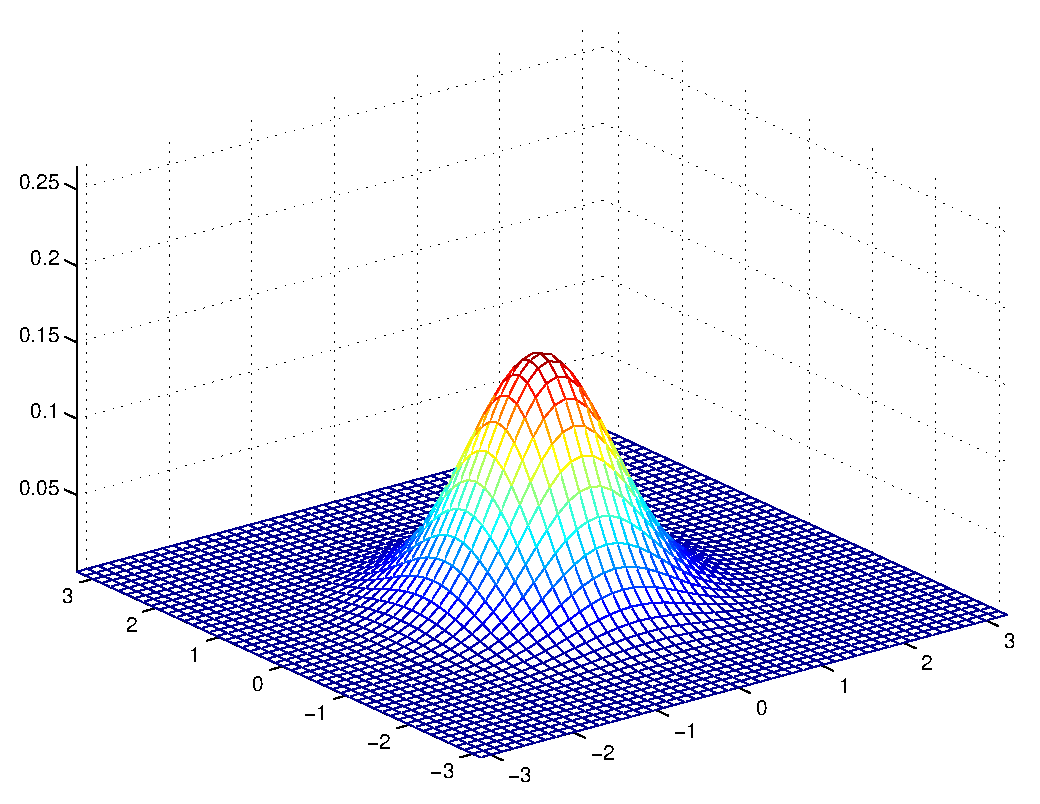
\includegraphics[width=0.32\textwidth]{gaussian_1_0_1.eps}
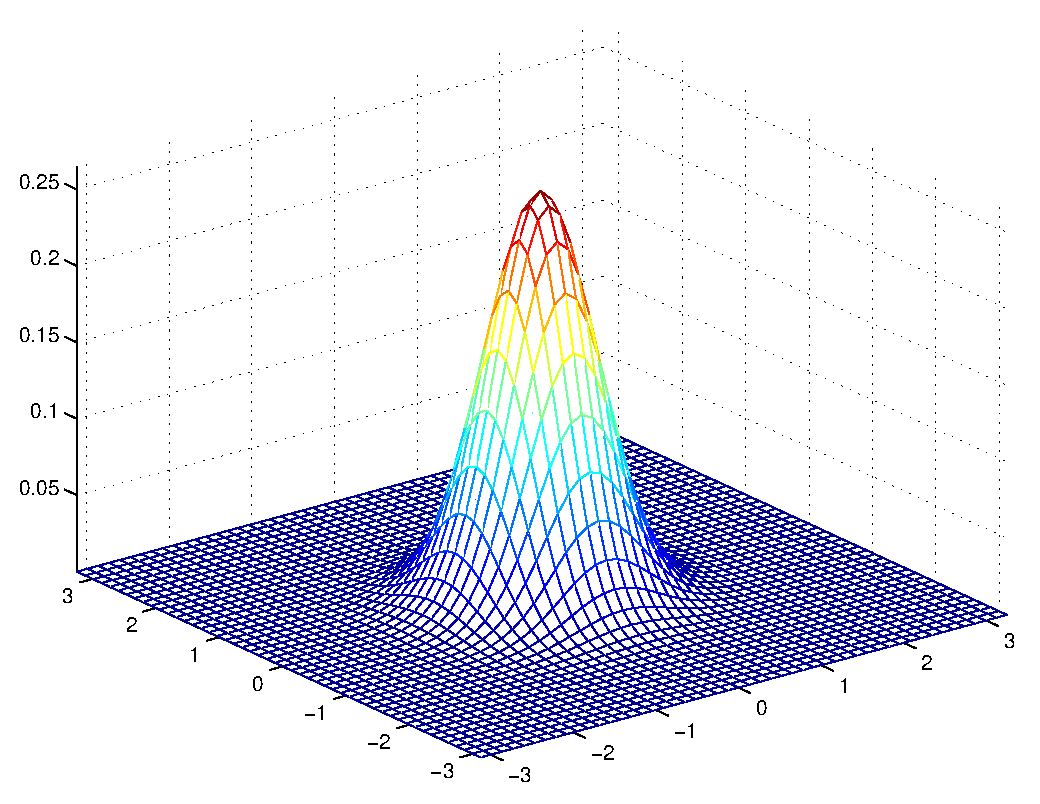
\includegraphics[width=0.32\textwidth]{gaussian_0-6_0_0-6.eps}
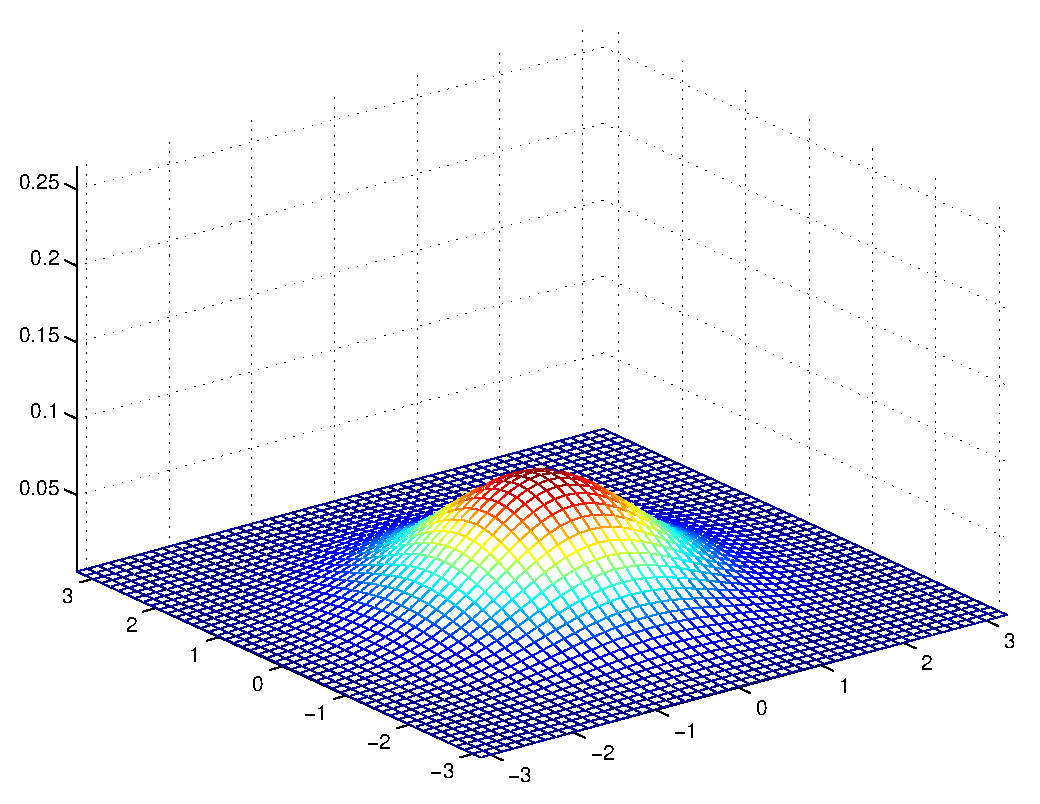
\includegraphics[width=0.32\textwidth]{gaussian_2_0_2.eps}
\end{figure}

%\threefigboxnolabel{gaussia{\di}_1_0_1.eps}{gaussia{\di}_0.6_0_0.6.eps}{gaussia{\di}_2_0_2.eps}

The left-most figure shows a Gaussian with mean zero (that is, the 2x1 zero-vector) and covariance matrix
$\Sigma = I$ (the 2x2 identity matrix).  A Gaussian with zero mean and identity covariance is
also called the {\bf standard normal distribution}.
The middle figure shows the density of a Gaussian with zero mean and $\Sigma = 0.6 I$; and in
the rightmost figure shows one with , $\Sigma = 2I$.  We see that as $\Sigma$ becomes larger,
the Gaussian becomes more ``spread-out,'' and as it becomes smaller, the distribution becomes
more ``compressed.''

Let's look at some more examples.


\threefigures{gaussian_1_0_1b.eps}{gaussian_1_0-5_1b.eps}{gaussian_1_0-8_1b.eps}
%\threefigboxnolabel{gaussia{\di}_1_0_1b.eps}{gaussia{\di}_1_0.5_1b.eps}{gaussia{\di}_1_0.8_1b.eps}

The figures above show Gaussians with mean 0, and with covariance matrices respectively
\[
\Sigma = \left[\begin{tabular}{cc} 1 & 0   \\ 0   &1 \end{tabular} \right];\;\;
\Sigma = \left[\begin{tabular}{cc} 1 & 0.5 \\ 0.5 &1 \end{tabular} \right];\;\;
\Sigma = \left[\begin{tabular}{cc} 1 & 0.8 \\ 0.8 &1 \end{tabular} \right].
\]
The leftmost figure shows the familiar standard normal distribution, and we see that as we increase the
off-diagonal entry in $\Sigma$, the density becomes more ``compressed'' towards the $45^\circ$ line
(given by $x_1 = x_2$).  We can see this more clearly when we look at the contours of
the same three densities:

\threefigures{gaussian_1_0_1con.eps}{gaussian_1_0-5_1con.eps}{gaussian_1_0-8_1con.eps}

Here's one last set of examples generated by varying $\Sigma$:

\threefigures{gaussian_1_-0-5_1con.eps}{gaussian_1_-0-8_1con.eps}{gaussian_3_0-8_1con.eps}

The plots above used, respectively,
\[
\Sigma = \left[\begin{tabular}{cc} 1 & -0.5 \\ -0.5 &1 \end{tabular} \right];\;\;
\Sigma = \left[\begin{tabular}{cc} 1 & -0.8 \\ -0.8 &1 \end{tabular} \right];\;\;
\Sigma = \left[\begin{tabular}{cc} 3 &  0.8 \\  0.8 &1 \end{tabular} \right].
\]
From the leftmost and middle figures, we see that by decreasing the off-diagonal elements of the
covariance matrix, the density now becomes ``compressed'' again, but in the opposite direction.
Lastly, as we vary the parameters, more generally the contours will form ellipses (the
rightmost figure showing an example).

As our last set of examples, fixing $\Sigma=I$, by varying $\mu$, we can also move the
mean of the density around.

\[
\threefigboxnolabel{gaussian_mu1.eps}{gaussian_mu2.eps}{gaussian_mu3.eps}
\]

The figures above were generated using $\Sigma = I$, and respectively
\[
\mu = \left[\begin{tabular}{c} 1 \\ 0 \end{tabular}\right]; \;\;
\mu = \left[\begin{tabular}{c} -0.5 \\ 0 \end{tabular}\right]; \;\;
\mu = \left[\begin{tabular}{c} -1 \\ -1.5 \end{tabular}\right].
\]


\subsection{The Gaussian Discriminant Analysis model}

When we have a classification problem in which the input features $x$ are continuous-valued
random variables, we can then use the Gaussian Discriminant Analysis (GDA) model, which
models $p(x|y)$ using a multivariate normal distribution.  The model is:
\begin{eqnarray*}
y &\sim& \Bernoulli(\phi)\\
x|y=0 &\sim& \calN(\mu_0, \Sigma) \\
x|y=1 &\sim& \calN(\mu_1, \Sigma) \\
\end{eqnarray*}
Writing out the distributions, this is:
\begin{eqnarray*}
p(y) &=& \phi^{y} (1-\phi)^{1-y} \\
p(x | y=0) &=& \frac{1}{(2\pi)^{\di/2} |\Sigma|^{1/2}} \exp\left(-\frac{1}{2}
                 (x-\mu_0)^T \Sigma^{-1} (x-\mu_0) \right) \\
p(x | y=1) &=& \frac{1}{(2\pi)^{\di/2} |\Sigma|^{1/2}} \exp\left(-\frac{1}{2}
                 (x-\mu_1)^T \Sigma^{-1} (x-\mu_1) \right) \\
\end{eqnarray*}
Here, the parameters of our model are $\phi$,
$\Sigma$, $\mu_0$ and $\mu_1$.
(Note that while there're two different mean vectors $\mu_0$ and $\mu_1$,
this model is usually applied using only one covariance matrix $\Sigma$.)
The log-likelihood of the data is given by
\begin{eqnarray*}
\ell(\phi, \mu_0, \mu_1, \Sigma) &=& \log \prod_{i=1}^\nexp p(x^{(i)} , y^{(i)}; \phi, \mu_0, \mu_1, \Sigma) \\
&=& \log \prod_{i=1}^\nexp p(x^{(i)} | y^{(i)}; \mu_0, \mu_1, \Sigma) p(y^{(i)}; \phi).
\end{eqnarray*}
By maximizing $\ell$ with respect to the parameters, we find the maximum likelihood
estimate of the parameters (see problem set 1) to be:
\begin{eqnarray*}
\phi &=& \frac{1}{\nexp} \sum_{i=1}^\nexp 1\{y^{(i)} = 1\} \\
\mu_0 &=& \frac{\sum_{i=1}^\nexp 1\{y^{(i)} = 0\} x^{(i)}}{\sum_{i=1}^\nexp 1\{y^{(i)} = 0\}} \\
\mu_1 &=& \frac{\sum_{i=1}^\nexp 1\{y^{(i)} = 1\} x^{(i)}}{\sum_{i=1}^\nexp 1\{y^{(i)} = 1\}} \\
\Sigma &=& \frac{1}{\nexp} \sum_{i=1}^\nexp (x^{(i)} - \mu_{y^{(i)}}) (x^{(i)} - \mu_{y^{(i)}})^T.
\end{eqnarray*}

Pictorially, what the algorithm is doing can be seen in as follows:

\begin{figure}[H]
\begin{center}
	\includegraphics[width=3in]{disgen3c.eps}
\end{center}
\end{figure}

%
%\begin{center}
%\epsfxsize=3in
%\epsffile{disgen3c.eps}
%\end{center}

Shown in the figure are the training set, as well as the contours of the
two Gaussian distributions that have been fit to the data in each of the
two classes.  Note that the two Gaussians have contours that are the same
shape and orientation, since they share a covariance matrix $\Sigma$, but
they have different means $\mu_0$ and $\mu_1$.  Also shown in the figure is
the straight line giving the decision boundary at which $p(y=1|x) = 0.5$.  On
one side of the boundary, we'll predict $y=1$ to be the most likely outcome, and
on the other side, we'll predict $y=0$.

\subsection{Discussion: GDA and logistic regression}

The GDA model has an interesting relationship to logistic regression.  If we view
the quantity $p(y=1|x;\phi, \mu_0, \mu_1, \Sigma)$ as a function of $x$, we'll
find that it can be expressed in the form
\[
p(y =1| x ; \phi, \Sigma, \mu_0, \mu_1) = \frac{1}{1+\exp(-\theta^Tx)},
\]
where $\theta$ is some appropriate function of $\phi, \Sigma, \mu_0, \mu_1$.\footnote{
This uses the convention of redefining the $x^{(i)}$'s on the right-hand-side to be
$(\di+1)$-dimensional vectors by adding the extra coordinate $x^{(i)}_0 = 1$; see
problem set 1.}  This is exactly the form that logistic regression---a discriminative algorithm---used to
model $p(y=1|x)$.

When would we prefer one model over another?  GDA and logistic regression will,
in general, give different decision boundaries when trained on the same dataset. Which is better?

We just argued that if $p(x|y)$ is multivariate gaussian (with shared $\Sigma$),
then $p(y|x)$ necessarily follows a logistic function.  The converse, however,
is not true; i.e., $p(y|x)$ being a logistic function does not imply
$p(x|y)$ is multivariate gaussian.  This shows that GDA makes \emph{stronger} modeling assumptions
about the data than does logistic regression.  It turns out that when these modeling
assumptions are correct, then GDA will find better fits to the data, and is a better model.
Specifically, when $p(x|y)$ is indeed gaussian (with shared $\Sigma$), then GDA is
{\bf asymptotically efficient}.  Informally, this means that in the limit of very large
training sets (large $\nexp$), there is no algorithm that is strictly better than GDA (in terms of,
say, how accurately they estimate $p(y|x)$).  In particular, it can be shown that in this
setting, GDA will be a better algorithm than logistic regression; and more generally,
even for small training set sizes, we would generally expect GDA to better.

In contrast, by making significantly weaker assumptions, logistic regression is also more
\emph{robust} and less sensitive to incorrect modeling assumptions.
There are many different sets of assumptions that would lead to $p(y|x)$ taking the form
of a logistic function.  For example, if
$x|y=0 \sim {\rm Poisson}(\lambda_0)$, and $x|y=1 \sim {\rm Poisson}(\lambda_1)$,
then $p(y|x)$ will be logistic.  Logistic regression will also work well on
Poisson data like this. But if we were to use GDA on such data---and fit Gaussian distributions to
such non-Gaussian data---then the results will be less predictable, and GDA may (or may not)
do well.

To summarize: GDA makes stronger modeling assumptions, and is more data efficient
(i.e., requires less training data to learn ``well'')
when the modeling assumptions are correct or at least approximately correct.  Logistic
regression makes weaker assumptions, and is significantly more robust to deviations
from modeling assumptions.  Specifically, when the data is indeed non-Gaussian, then
in the limit of large datasets, logistic regression will almost always do better than
GDA.  For this reason, in practice logistic regression is used more often than GDA.
(Some related considerations about discriminative vs.  generative models also apply for
the Naive Bayes algorithm that we discuss next, but the Naive Bayes algorithm is still
considered a very good, and is certainly also a very popular, classification algorithm.)

%It is still a matter of debate among machine learning researchers exactly how
%much better either algorithm is in either setting, but in problems when $x$
%is fairly low-dimensional and where there is abundant training data, logistic
%regression is usually used.


\section{Naive Bayes}

In GDA, the feature vectors $x$ were continuous, real-valued vectors.  Let's now talk
about a different learning algorithm in which the $x_j$'s are discrete-valued.

For our motivating example, consider building an email spam filter using machine
learning.  Here, we wish to classify messages according to whether they are
unsolicited commercial (spam) email, or non-spam email.  After learning to do this,
we can then have our mail reader automatically filter out the spam messages and perhaps
place them in a separate mail folder.  Classifying emails is one example of a broader
set of problems called {\bf text classification}.

Let's say we have a training set (a set of emails labeled as spam or non-spam).
We'll begin our construction of our spam filter by specifying the features $x_j$ used
to represent an email.

We will represent an email via a feature vector whose length is equal to the number
of words in the dictionary.  Specifically, if an email contains the $j$-th word of the
dictionary, then we will set $x_j$ = 1; otherwise, we let $x_j=0$.  For instance,
the vector
\[
x = \left[\begin{tabular}{c} 1 \\ 0 \\ 0 \\ \vdots \\ 1 \\ \vdots \\ 0 \end{tabular} \right]
\;\;\;\begin{tabular}{l} a \\ aardvark \\ aardwolf \\ \vdots \\ buy \\ \vdots \\ zygmurgy \end{tabular}
\]
is used to represent an email that contains the words ``a'' and ``buy,'' but
not ``aardvark,'' ``aardwolf'' or ``zygmurgy.''\footnote{Actually,
rather than looking through an English dictionary for the list of all English words,
%we may simply take the $\di$ most commonly occurring words in English (for some large
%value of $\di$), or
in practice
it is more common to look through our training set and encode in our feature vector
only the words that occur at least once there.  Apart from reducing the number of
words modeled and hence reducing our computational and space requirements, this also
has the advantage of allowing us to model/include as a feature many words that may appear in your
email (such as ``cs229'') but that you won't find in a dictionary.
Sometimes (as in the homework),
we also exclude the very high frequency words (which will be words like ``the,'' ``of,'' ``and'';
these high frequency, ``content free'' words are called {\bf stop words}) since they occur in so
many documents and do little to indicate whether an email is spam or non-spam.}
The set of words encoded into the feature vector is called the {\bf vocabulary}, so
the dimension of $x$ is equal to the size of the vocabulary.
%HERE: Above para needs rephrasing?


Having chosen our feature vector, we now want to build a generative model.
So, we have to model  $p(x|y)$.  But if we have, say, a vocabulary of 50000 words,
then $x \in \{0,1\}^{50000}$ ($x$ is a 50000-dimensional vector of 0's and 1's),
and if we were to model $x$ explicitly with a multinomial
distribution over the $2^{50000}$ possible outcomes, then we'd end up with a
$(2^{50000}-1)$-dimensional parameter vector.  This is clearly too many parameters.

To model $p(x|y)$, we will therefore make a very strong assumption.  We will
assume that the $x_i$'s are conditionally independent given $y$.
This assumption is called the {\bf Naive Bayes (NB) assumption}, and the
resulting algorithm is called the {\bf Naive Bayes classifier}.
For instance, if $y=1$ means spam email; ``buy'' is word 2087 and ``price'' is word 39831;
then we are assuming that if I tell you $y=1$ (that a particular piece of email is spam), then
knowledge of $x_{2087}$ (knowledge of whether ``buy'' appears in the message) will have
no effect on your beliefs about the value of $x_{39831}$ (whether ``price'' appears).
More formally, this can be written $p(x_{2087}|y) = p(x_{2087}|y, x_{39831})$.
(Note that this is \emph{not} the same as saying that $x_{2087}$ and $x_{39831}$
are independent, which would have been written  ``$p(x_{2087}) = p(x_{2087}| x_{39831})$''; rather,
we are only assuming that $x_{2087}$ and $x_{39831}$ are conditionally independent \emph{given} $y$.)

We now have:
\begin{eqnarray*}
p(x_1,\ldots,x_{50000}|y) \hbox to -1.2in{}&&\\
&=& p(x_1|y) p(x_2|y, x_1) p(x_3|y, x_1, x_2) \cdots p(x_{50000}|y, x_1,\ldots, x_{49999}) \\
&=&p(x_1|y) p(x_2|y) p(x_3|y) \cdots p(x_{50000}|y) \\
&=& \prod_{j=1}^\di p(x_j|y)
\end{eqnarray*}
The first equality simply follows from the usual properties of probabilities,
and the second equality used the NB assumption.
We note that even though the Naive Bayes assumption is an extremely strong
assumptions, the resulting algorithm works well on many problems.

Our model is parameterized by $\phi_{j|y=1} = p(x_j=1 | y=1)$,
$\phi_{j|y=0} = p(x_j=1 | y=0)$,
and $\phi_y = p(y=1)$.  As usual, given a training set $\{(\xsi, \ysi); i=1,\ldots,\nexp\}$, we
can write down the joint likelihood of the data:
\[
\calL(\phi_y, \phi_{j|y=0}, \phi_{j|y=1}) = \prod_{i=1}^\nexp p(\xsi, \ysi).
\]
Maximizing this with respect to $\phi_y, \phi_{j|y=0}$ and $\phi_{j|y=1}$ gives
the maximum likelihood estimates:
\begin{eqnarray*}
\phi_{j|y=1} &=& \frac{\sum_{i=1}^\nexp 1\{x^{(i)}_j =1 \wedge \ysi=1\}}{\sum_{i=1}^\nexp 1\{\ysi=1\}} \\
\phi_{j|y=0} &=& \frac{\sum_{i=1}^\nexp 1\{x^{(i)}_j =1 \wedge \ysi=0\}}{\sum_{i=1}^\nexp 1\{\ysi=0\}} \\
\phi_y &=& \frac{\sum_{i=1}^\nexp 1\{\ysi = 1\}}{\nexp}
\end{eqnarray*}
In the equations above, the ``$\wedge$'' symbol means ``and.''  The parameters have
a very natural interpretation.  For instance, $\phi_{j|y=1}$ is just the fraction of
the spam ($y=1$) emails in which word $j$ does appear.

Having fit all these parameters, to make a prediction on a new example with features $x$,
we then simply calculate
\begin{eqnarray*}
p(y=1|x) &=& \frac{p(x|y=1) p(y=1)}{p(x)} \\
&=& \frac{\left(\prod_{j=1}^\di p(x_j|y=1)\right) p(y=1)}{\left(\prod_{j=1}^\di p(x_j|y=1)\right) p(y=1) + \left(\prod_{j=1}^\di p(x_j|y=0)\right) p(y=0)},
\end{eqnarray*}
and pick whichever class has the higher posterior probability.

Lastly, we note that while we have developed the Naive Bayes algorithm mainly for the
case of problems where the features $x_j$ are binary-valued, the generalization to
where $x_j$ can take values in $\{1, 2, \ldots, k_j\}$
is straightforward.  Here, we would simply model $p(x_j|y)$ as multinomial rather than as Bernoulli.
Indeed,
even if some original input attribute
(say, the living area of a house,
as in our earlier example)
were continuous valued, it is quite common to {\bf discretize} it---that is, turn it into
a small set of discrete values---and apply Naive Bayes.  For instance, if we use some
feature $x_j$ to represent living area, we might discretize the continuous values as follows:

\begin{tabular}{c|c|c|c|c|c}
Living area (sq. feet) & $<$ 400 & 400-800 & 800-1200 & 1200-1600 & $>$1600 \\ \hline
$x_i$ & 1 & 2 & 3 & 4 & 5 \\
\end{tabular}

Thus, for a house with living area 890 square feet, we would set the value of
the corresponding feature $x_j$ to 3.  We can then apply the Naive Bayes algorithm, and model
$p(x_j|y)$ with a multinomial distribution, as described previously.  When the original,
continuous-valued attributes are not well-modeled by a multivariate normal distribution, discretizing the
features and using Naive Bayes (instead of GDA) will often result in a better classifier.

\subsection{Laplace smoothing}

The Naive Bayes algorithm as we have described it will work fairly well for many problems,
but there is a simple change that makes it work much better, especially for text classification.
Let's briefly discuss a problem with the algorithm in its current form, and then talk about
how we can fix it.

Consider spam/email classification, and let's suppose that, we are in the year of 20xx, after completing CS229 and having
done excellent work on the project, you decide around May 20xx to submit
work you did to the NeurIPS conference for publication.\footnote{NeurIPS is one of the top machine learning conferences.  The deadline for submitting a
paper is typically in May-June.}  Because you end up discussing the conference in
your emails, you also start getting messages with the word ``neurips'' in it.  But this is your first
NeurIPS paper, and until this time, you had not previously seen any emails containing the word ``neurips'';
in particular ``neurips'' did not ever appear in your training set of spam/non-spam emails.
Assuming that ``neurips'' was the
35000th word in the dictionary, your Naive Bayes spam filter therefore had picked its
maximum likelihood estimates of the parameters $\phi_{35000|y}$ to be
\begin{eqnarray*}
\phi_{35000|y=1} &=& \frac{\sum_{i=1}^\nexp 1\{x^{(i)}_{35000} =1 \wedge \ysi=1\}}{\sum_{i=1}^\nexp 1\{\ysi=1\}} = 0\\
\phi_{35000|y=0} &=& \frac{\sum_{i=1}^\nexp 1\{x^{(i)}_{35000} =1 \wedge \ysi=0\}}{\sum_{i=1}^\nexp 1\{\ysi=0\}} = 0
\end{eqnarray*}
I.e., because it has never seen ``neurips'' before in either spam or non-spam training examples, it thinks
the probability of seeing it in either type of email is zero.  Hence, when trying to decide if
one of these messages containing ``neurips'' is spam, it calculates the
class posterior probabilities, and obtains
\begin{eqnarray*}
p(y=1|x)
&=& \frac{\prod_{j=1}^\di p(x_j|y=1) p(y=1)}{\prod_{j=1}^\di p(x_j|y=1) p(y=1) + \prod_{j=1}^\di p(x_j|y=0) p(y=0)} \\
&=& \frac{0}{0}.
\end{eqnarray*}
This is because each of the terms ``$\prod_{j=1}^\di p(x_j|y)$'' includes a term $p(x_{35000}|y) = 0$ that
is multiplied into it.  Hence, our algorithm obtains $0/0$, and doesn't know how to make a prediction.

Stating the problem more broadly, it is statistically a bad idea to estimate the probability of some event to be zero
just because you haven't seen it before in your finite training set. Take the problem of estimating
the mean of a multinomial random variable $z$ taking values in $\{1, \ldots, k\}$.  We can parameterize
our multinomial with $\phi_j = p(z=j)$.  Given a set of $\nexp$ independent observations $\{z^{(1)}, \ldots, z^{(\nexp)}\}$, the
maximum likelihood estimates are given by
\[
\phi_j = \frac{\sum_{i=1}^\nexp 1\{z^{(i)}=j\}}{\nexp}.
\]
As we saw previously, if we were to use these maximum likelihood estimates, then some of the $\phi_j$'s might
end up as zero, which was a problem.
To avoid this, we can use {\bf Laplace smoothing}, which replaces the above estimate with
\[
\phi_j = \frac{1 + \sum_{i=1}^\nexp 1\{z^{(i)} = j\}}{k + \nexp}.
\]
Here, we've added 1 to the numerator, and $k$ to the denominator.
Note that $\sum_{j=1}^k \phi_j = 1$ still holds (check this yourself!), which is a desirable property since
the $\phi_j$'s are estimates for probabilities that we know must sum to 1.  Also, $\phi_j \neq 0$ for all values
of $j$, solving our problem of probabilities being estimated as zero.  Under certain (arguably quite strong) conditions, it can be shown that the Laplace
smoothing actually gives the optimal estimator of the $\phi_j$'s.

Returning to our Naive Bayes classifier, with Laplace smoothing, we therefore obtain the
following estimates of the parameters:
\begin{eqnarray*}
\phi_{j|y=1} &=& \frac{1 + \sum_{i=1}^\nexp 1\{x^{(i)}_j =1 \wedge \ysi=1\}}{2 + \sum_{i=1}^\nexp 1\{\ysi=1\}} \\
\phi_{j|y=0} &=& \frac{1 + \sum_{i=1}^\nexp 1\{x^{(i)}_j =1 \wedge \ysi=0\}}{2 + \sum_{i=1}^\nexp 1\{\ysi=0\}} \\
\end{eqnarray*}
(In practice, it usually doesn't matter much whether we apply Laplace smoothing to $\phi_y$ or not,
since we will typically have a fair fraction each of spam and non-spam messages, so
$\phi_y$ will be a reasonable estimate of $p(y=1)$ and will be quite far from 0 anyway.)


\subsection{Event models for text classification}

To close off our discussion of generative learning algorithms, let's talk about one more
model that is specifically for text classification.  While Naive Bayes as we've presented
it will work well for many classification problems, for text classification, there is
a related model that does even better.

In the specific context of text classification, Naive Bayes as presented uses the what's
called the {\bf Bernoulli event model} (or sometimes {\bf multi-variate Bernoulli event model}).  In this model, we assumed that the
way an email is generated is that first it is randomly determined (according to the class
priors $p(y)$) whether a spammer or non-spammer will send you your next message.  Then,
the person sending the email runs through the dictionary, deciding whether to include each word $j$
in that email independently and according to the probabilities $p(x_j=1|y) = \phi_{j|y}$.  Thus,
the probability of a message was given by $p(y) \prod_{j=1}^\di p(x_j|y)$.

Here's a different model, called the {\bf Multinomial event model}.  To describe this model, we
will use a different notation and set of features for representing emails.  We let $x_j$ denote the identity
of the $j$-th word in the email.  Thus, $x_j$ is now an integer taking values in $\{1,\ldots, |V|\}$,
where $|V|$ is the size of our vocabulary (dictionary).  An email of $\di$ words
is now represented by a vector $(x_1, x_2, \ldots, x_{\di})$ of length $\di$; note that $\di$ can
vary for different documents.  For instance, if an email starts with ``A NeurIPS \dots,'' then
$x_1=1$ (``a'' is the first word in the dictionary), and $x_2 = 35000$ (if ``neurips'' is the
35000th word in the dictionary).

In the multinomial event model, we assume that the way an email is generated is via
a random process in which spam/non-spam is first determined (according to $p(y)$) as before.  Then,
the sender of the email writes the email by first generating $x_1$ from some multinomial
distribution over words ($p(x_1|y)$).  Next, the second word $x_2$ is chosen independently
of $x_1$ but from the same multinomial distribution, and similarly for $x_3$, $x_4$, and so on, until
all $\di$ words of the email have been generated.
Thus, the overall probability of a message is given by $p(y) \prod_{j=1}^\di p(x_j|y)$.  Note
that this formula looks like the one we had earlier for the probability of a message under the
Bernoulli event model, but that the terms in the formula now mean very different things.
In particular $x_j|y$ is now a multinomial, rather than a Bernoulli distribution.

% The reasons that the multinomial event model does better are quite subtle, and are still some
% matter of debate among machine learning researchers.   Certainly however, one disadvantage
% of the multi-variate Bernoulli model is that it fails to take into account the number of times
% words appear in a document (i.e., whether ``buy'' occurs one time or ten times in an email,
% it is encoded as some same $x_{2087}=1$ feature).
% %, whereas the multinomial model may make
% %different predictions depending on the number of times each word occurs.

The parameters for our new model are $\phi_y = p(y)$ as before,
$\phi_{k|y=1} = p(x_j=k|y=1)$ (for any $j$)
and $\phi_{k|y=0} = p(x_j=k|y=0)$.
Note that we have assumed that $p(x_j|y)$ is the same for all values of $j$ (i.e., that the
distribution according to which a word is generated does not depend on its position $j$
within the email).

If we are given a training set
$\{(\xsi, \ysi); i=1,\ldots,\nexp\}$ where $\xsi =
(x^{(i)}_1, x^{(i)}_2, \ldots, x^{(i)}_{\di_i})$ (here, ${\di}_i$ is the number of words in the $i$-training
example), the likelihood of the data is given by
\begin{eqnarray*}
\calL(\phi_y, \phi_{k|y=0}, \phi_{k|y=1}) &=& \prod_{i=1}^\nexp p(\xsi, \ysi) \\
&=& \prod_{i=1}^\nexp \left(\prod_{j=1}^{\di_i} p(x^{(i)}_j|y ;  \phi_{k|y=0}, \phi_{k|y=1}) \right) p(\ysi ; \phi_y).
\end{eqnarray*}
Maximizing this yields the maximum likelihood estimates of the parameters:
\begin{eqnarray*}
\phi_{k|y=1} &=& \frac{\sum_{i=1}^\nexp \sum_{j=1}^{\di_i} 1\{x_j^{(i)} = k \wedge \ysi = 1\}}{\sum_{i=1}^\nexp 1\{\ysi=1\}{\di}_i} \\
\phi_{k|y=0} &=& \frac{\sum_{i=1}^\nexp \sum_{j=1}^{\di_i} 1\{x_j^{(i)} = k \wedge \ysi = 0\}}{\sum_{i=1}^\nexp 1\{\ysi=0\}{\di}_i}\\
\phi_y &=& \frac{\sum_{i=1}^\nexp 1\{\ysi = 1\}}{\nexp}.
\end{eqnarray*}
If we were to apply Laplace smoothing (which is needed in practice for good performance) when
estimating $\phi_{k|y=0}$ and $\phi_{k|y=1}$, we add 1 to the numerators and $|V|$ to the
denominators, and obtain:
\begin{eqnarray*}
       \phi_{k|y=1} &=& \frac{1 + \sum_{i=1}^\nexp \sum_{j=1}^{\di_i} 1\{x_j^{(i)} = k \wedge \ysi = 1\}}{|V| + \sum_{i=1}^\nexp 1\{\ysi=1\}{\di}_i} \\
       \phi_{k|y=0} &=& \frac{1 + \sum_{i=1}^\nexp \sum_{j=1}^{\di_i} 1\{x_j^{(i)} = k \wedge \ysi = 0\}}{|V| + \sum_{i=1}^\nexp 1\{\ysi=0\}{\di}_i}.
\end{eqnarray*}
While not necessarily the very best classification algorithm, the Naive Bayes classifier
often works surprisingly well.  It is often also a very good ``first thing to try,''
given its simplicity and ease of implementation.

%\begin{center}
%\epsfxsize=3in
%\epsffile{foo.eps}
%\end{center}

\end{document}
